\documentclass{article} % For LaTeX2e
\usepackage{iclr2018_conference,times}
\usepackage{url}
\usepackage{amsthm}
\usepackage{algorithm}
\usepackage{algorithmic}
\usepackage{times}
\usepackage{graphicx}
\usepackage{color}
\usepackage{amsmath}
\usepackage{amsfonts}
\usepackage{url}
\usepackage{textcomp}
\usepackage{amsthm}
\usepackage{float}

\frenchspacing

\def\presentationmode{1}

\def\beginFrame#1{\if\presentationmode1 \begin{frame}{#1} \else \fi}
\def\endFrame{\if\presentationmode1 \end{frame} \else \fi}

\newcommand{\mat}[1]{\mathrm{\mathbf{#1}}}
\newcommand{\vect}[1]{\mathrm{\mathbf{#1}}}
\newcommand{\fros}[1]{\left\| #1 \right\|_\mathrm{F}^2}
\newcommand{\Expect}[2]{\mathbb{E}_{#1}\left[ #2 \right]}
\newcommand{\KL}[2]{ \mathrm{KL}\left( #1 \| #2 \right) }
\newcommand{\Real}{\mathbb{R}}
\newcommand{\T}{\mathrm{T}}
\newcommand{\tr}{\mathrm{tr}}
\newcommand{\sigmoid}{\sigma}
\newcommand{\attention}{\vect{g}}
\def\attentionwithouti{g_2, \dots, g_k}
%\def\attentionwithouti{\boldsymbol{\gamma}_{i}}
\newcommand{\attraction}{\vect{h}}

\def\x{\vect{x}}
\def\y{\vect{y}}
\def\h{\vect{h}}
\def\g{\vect{g}}
\def\s{\vect{s}}
\def\c{\vect{c}}
\def\A{\mathcal{A}}
\def\S{\mathcal{S}}
\def\R{\mathcal{R}}
\def\Trans{\mathcal{T}}
\def\Observations{\Omega}
\def\ObProb{\mathcal{O}}
\def\E{\mathcal{E}}
\def\deriv#1#2{ \frac{\partial #2}{ \partial #1 } }
\def\derivN#1#2#3{ \frac{\partial^{#1} #3}{ \partial #2^{#1} } }
\def\grad#1#2{ \deriv{#1}{#2} }
\def\gradN#1#2#3{ \derivN{#1}{#2}{#3} }
\def\Grad#1#2{ \nabla_{#1} {#2} }
\def\obs{\vect{o}}
\def\u{{\boldsymbol{b}}}
\def\w{{\boldsymbol{\alpha}}}
\def\vmu{{\boldsymbol{\mu}}}
\def\v{\vect{v}}
\def\g{\attention}
\def\h{\attraction}
\def\G{\mat{G}}
\def\op{}
%\def\Qg{Q^{\mathrm{g}}}
%\def\ug{\vect{u}^{\mathrm{g}}}
\def\Qg{Q}
\def\ug{\u}
\def\params{{\boldsymbol{\theta}}}
\def\Params{{\boldsymbol{\Theta}}}
\def\opt#1{{\hat{#1}}}

\newcommand{\argmax}{\mathop{\rm argmax}\limits}
\newcommand{\argmin}{\mathop{\rm argmin}\limits}


%\def\costof#1{C(#1)}
\def\costof#1{\mathrm{C}[{#1}]}
\def\budget{B}
\def\cost{c}
\def\vcost{\vect{\cost}}
\def\costat#1{\cost_{#1}}
\def\costi{c_i}
\def\unit{\vect{e}}
\def\state{\s}
\def\action{a}
\def\rewards{y}

\def\sumk#1{\sum_{#1=1}^k}
\def\Si{\sumk{i}}
\def\Sj{\sumk{j}}

\def\vcatout{\tilde{\vect{h}}}
\def\catout{\tilde{h}_i}
\def\catoutj{\tilde{h}_j}
\def\changeof#1{\Delta #1}

\def\vcatin{\vect{h}}
\def\catin{h_{i}}
\def\catinj{h_{j}}

\def\vcatbias{\vect{h}_i}
\def\catbias{\mu_i}
\def\catbiasj{\mu_j}

\def\qbias{q_i}
\def\vqbias{\mathbf{q}}
\def\qin{Q}

\def\ebias{e_{-i}}
\def\ein{e}
\def\changeofebias{{\changeof\qbias} \left[ \changeof\qbias + 2 \TDerror{\qin} \right]}
%\def\changeofebias{{\changeof\qbias}\left( \changeof\qbias + 2 \delta_t \right)}

\def\regret{\rho_{-i}}
%\def\TDerror#1{E_{\mathrm{TD}}\left({#1}\right)}
\def\TDerror#1{\delta}


\def\prA{p(\rewards|\state, \action, \params, \g)}
\def\LLAttention{\log \prA}

\def\Square#1{\left[ #1 \right]^2}

\def\ReplayMemory{\mathcal{D}}
\def\play{\s_t, a_t, r_t, \s_{t+1}}
\def\Play{(\play)}
\def\pl{\mathsf{d}_t}
\def\Replays#1{\Expect{ \pl \sim \ReplayMemory}{#1}}

\def\bUpdate#1{p(o_{t+1}|s_${#1},a_t) \sum_i p(s_{#1}|s_i, a_t) b_{t}^i}
\def\beliefState#1{ \vect{b}_{#1} }

\def\const{\mathrm{const.}}
\def\test{_\mathrm{test}}
\def\train{_\mathrm{train}}
\def\bs{\boldsymbol}
\def\etal#1{{et al.} (\citeyear{#1})}
\def\Etal{{et al.}}
\def\Long{1}
\def\eg{e.g., }

\def\eAt#1{e_{#1}}
\def\eBase{\eAt{\one}}
\def\one{\mathbf{1}}
\def\zero{\mathbf{0}}
\def\unit#1{\vect{u}_{#1}}
\def\eChange#1{ \Delta e_{#1} }

\def\ask{q}


% probability
\def\prob#1{p\left(#1\right)}
\def\prob#1#2{p\left(#1 \mid #2 \right)}

\def\deprecated{\alert{[Deprecated]}}
\def\softmax{\mathrm{softmax}}


\newcommand{\penalvec}[3]{ \frac{1}{2 \sigma_#1^2} \sum_{#2=1}^{#3} \vect{#1}_{#2}^\T  \vect{#1}_{#2} }

\newcommand{\CON}{\color{red}}
%\newcommand{\CON}{\color{black}}
\newcommand{\COFF}{\color{black}}

%\newcommand{\CON}{\color{red} -------- My modification starts from here. ------- \color{black}}
%\newcommand{\CON}{\color{black}}
%\newcommand{\COFF}{\color{red} -------- My modification ends here. ------- \color{black} }


\newtheorem{thm}{Theorem}[section]
\newtheorem{coro}{Corollary}[section]
\newtheorem{prf}{Proof}
\newtheorem{defn}{Definition}




%=================================
% Paper specific
%=================================

\def\neuralnet{\mathfrak{G}}
\def\units{\mathcal{V}}
\def\edges{\mathcal{E}}
\def\unitAt#1{v_{#1}}
\def\unit{\unitAt{i}}
\def\followees{N^\mathrm{in}_i}
\def\followers{N^\mathrm{out}_i}
\def\friends{N_i}
\def\rewardAt#1{R_{#1}}
\def\reward{\rewardAt{it}}



\title{Neuron as an Agent}

%\author{Shohei Ohsawa, Kei Akuzawa, Yusuke Iwasawa \& Yutaka Matsuo \\
%The University of Tokyo\\
%7 Chome-3-1 Hongo, Bunkyo, Tokyo \\
%\texttt{ohsawa@weblab.t.u-tokyo.ac.jp} \\
%}
\author{Anonymous}

\newcommand{\fix}{\marginpar{FIX}}
\newcommand{\new}{\marginpar{NEW}}

\begin{document}

\maketitle

\begin{abstract}
Communication methods on multi-agent reinforcement learning (MARL) so far relies on a trusted third party (TTP) which distributes incentive to agents, and hence cannot be applied into a peer-to-peer environment.
We propose {\em Neuron as an Agent} (NaaA) for incentive distribution in MARL without TTP with two key ideas:
(i) inter-agent reward distribution and (ii) auction theory.
The reason why we introduce auction theory is inter-agent reward distribution is insufficient for optimization.
An agent in NaaA maximizes its profit, difference between reward and cost.
As a theoretical result, we show that the auction mechanism has an agent autonomously evaluates counterfactual return as other agent's value.
NaaA enables us to trade of representation in peer-to-peer and regard a unit in a neural network as an agent ultimately.
Finally, we confirm that optimization with the framework of NaaA leads to better performance of RL, with numerical experiments.
Specifically, we use a single-agent environment from Open AI gym, and a multi-agent environment from ViZDoom.
\end{abstract}

%We propose {\em Neuron as an Agent} (NaaA) as a novel framework for deep multi-agent reinforcement learning (MARL),
%which incorporates all neural network units as agents and optimizes the reward distribution. % as a MARL problem.
%NaaA deals with reward distribution among the agents by combining MARL with economics.
%As a theoretical result, we demonstrate that the agent obeys the system to maximize its {\em counterfactual return} as the Nash equilibrium of the mechanism.
%Subsequently, we show that learning counterfactual returns leads the model to learning optimal topology among units, and improves performance of a single-agent RL task.
%We propose {\em adaptive dropconnect}, a natural extension of dropconnect.

\section{Introduction}

%===========================================================================================
% Motivation
%===========================================================================================
After intelligence with reinforcement learning beat humans \citep{tesauro1995temporal,mnih2015human,silver2016mastering}, reinforcement learning has been expected to be applied into industry such as stock trade, autonomous cars, smart grid and IoT. 
In a world which realized the industrial application in the future, various types of companies will own their agents to improve their revenue.
The situation can be regarded as one that each agent are independently solving problems of partially observed Markov decision process (POMDP).

Although agents in the companies are closed to maximize their own reward, if the agents exchange their own information each other, 
entire revenue will be improved more than individuals.
Using economic metaphor, similarly to a supply chain of diamond from a company which collects raw material, one which processes it to one which sells it, if we can realize representation learning in the each layers as social division, a single company can yield revenue more than one by itself. %in the case the company does it by itself.
Thus, this paper aims to realize a society in which stakeholders which can have a conflict of interest trade their own information.

We regard the situation as communication in multi-agent reinforcement learning (MARL), addressed by several existing methods such as R/DIAL \citep{foerster2016learning} and CommNet \citep{sukhbaatar2016learning}.
CommNet is a state-of-the-art of MARL which considers communication among agents, 
and the feature is learning among agents with backpropagation.

In the case when we are trying to consider MARL in which different stakeholders make different agents which communicate each other, it needs design of incentive distribution (e.g., monetary payment) and a framework without {\em trusted third party} (TTP).
TTP is a neutral administrator which assumes distribution of reward for all the participants, supposed implicitly by most of existing literatures with regard to MARL \citep{agogino2006quicr,foerster2016learning,sukhbaatar2016learning}.
While TTP is required to be neutral against all the participants,
several configuration of peer-to-peer trade such as inter-industry and -country trade cannot prepare TTP.
If untrusted third party assumes reward distribution, it can undesirably make reward for partial participants higher than necessity.

To the best of our knowledge, no existing literatures discuss the reward distribution on the configuration above.
Since CommNet assumes an environment which distributes a uniform reward to all the agents, 
in the case distributing limited reward in supply such as money, it causes {\em Tragedy of the Commons} \citep{lloyd1833two} in which contributing agents' reward will reduce due to participant of free riders.
Although there are several MARL methods which distributes reward depends on their contribution such as QUICR \citep{agogino2006quicr} and COMA \citep{sukhbaatar2016learning}, they suppose the existence of TTP, and hence it cannot be applied into our situation.

%===========================================================================================
% Objective
%===========================================================================================

Our proposed method, {\em Neuron as an Agent} (NaaA) extends CommNet to realize incentive distribution
in MARL without TTP with two key ideas: (i) inter-agent reward distribution and (ii) auction theory.
The reason why we introduce auction theory is inter-agent reward distribution is insufficient for optimization.
An agent in NaaA maximizes {\em profit}, difference between reward which it receives and cost which it redistributes to other agents.
If we optimize the framework naively, we obtain a trivial solution that agents make their cost zero to maximize the profit.
Then, NaaA employs game design with auction theory to keep cost being smaller than necessity.
As a theoretical result, we show that an agent autonomously evaluates {\em counterfactual return} as other agent's value.
Counterfactual return equals to discounted cumulative sum of counterfactual reward \citep{agogino2006quicr} which QUICR and COMA distribute.
NaaA realizes reward distribution which make it pareto improvement more than inter-agent reward distribution.

NaaA enables us to trade of representation in peer-to-peer and regard a unit in a neural network as an agent ultimately.
As NaaA can regard a unit as an agent without loss of generality indeed, this paper uses the setting.
We illustrate the concept proposed method in Fig. 1 (TBD).

In the experiment, we use an environment which extends ViZDoom \citep{kempka2016vizdoom}, a POMDP environemnt, to MARL.
We put two agents in the environment.
The one is a cameraman who send information, and the another one is a main player to defeat enemies with a gun.
We confirm that the cameraman learns cooperative action to send information in dead angle, behind of main player, and outperform CommNet in score.

% Organization
The remaining part of this paper is organized as follows. 
First, we describe the two key ideas: inter-agent reward distribution and auction theory. 
After introducing related works, we show the experimental result in ViZDoom.
Next, we show Adapritve DropConnect as a further application. Then we perform discussion and conclude this paper.

%\section{Background}
First, we consider a POMDP environment in which a single agent acts.
The POMDP environment is a seven-tuple $(\S, \A, \Trans, \R, \Observations, \ObProb, \gamma)$,
where $\S$ represents a set of states, $\A$ stands for a set of actions, $\Trans$ denotes a transitive probability, 
$\Observations$ represents a possible set of observations, $\ObProb$ denotes a set of observation probability, and
$\gamma$ is the discount rate.
An agent partially predicts state $h \in \S$ through an observation $s \in \Observations$.
Generally, $s$ has higher dimensions than $h$, and is complex.
For example, although Atari 2600 has a read only memory (RAM) as the true state, which contains 128 bytes,
the generated image from that $s$ has more than 10,000 dimensions.
Therefore, DQN and DRQN abstract $s$, and create original state representation to predict good action efficiently.
(Although the original paper of DQN assumes MDP, the paper of DRQN pointed out that the environment is POMDP).
Although DQN does not address the state transition directly because it is model-free method, 
some interpretations hold that the hidden state representation is learned in the previous layer of the output layer \citep{zahavy2016graying}
Using the method below, we assume that the agent chooses an action through a neural network.

%TODO: POSG

The design of NaaA is inspired by neuroscience.
A neuron in a neurocircuit consumes adenosine triphosphate (ATP) supplied from connected astrocytes.
The astrocyte is a glia cell, which forms the structure of a brain. It supplies fuel from the vessel.
Because the amount of ATP is constrained, the discarded neuron will become extinct with execution of apoptosis.
Also, because apoptosis of a neuron is restrained by neurotrophins (NTFs) such as nerve growth factor (NGF) and brain-derived neurotrophic factor (BDNF),
neurons which can obtain much NTF will live.
The perspective of interpreting a neuron as an independent living object is known as neural Darwinism \citep{edelman1987neural}.

\section{Neuron as an Agent}
TODO: Show the figure.

A typical artificial neural network is a directed graph $\neuralnet = (\units, \edges)$ among the units.
$\units = \{\unitAt{1}, \dots, \unitAt{N}\}$ is a set of the units, and $\edges \subset \units^2$ is a set of edge indicating connection between two units.
If $(\unit, \unitAt{j}) \in \edges$, then connection $\unit \rightarrow \unitAt{j}$ holds, indicating $\unitAt{j}$ observes activation of $\unit$.
We denote activation of the unit $\unit$ at time $t$ as $x_{it} \in \Real$.
Also, we denote a set of units which unit $i$ connects to as $\followers = \{j | (\unit, \unitAt{j}) \in \edges \}$, and a set of units which unit $i$ is connected from is $\followees = \{j | (\unitAt{j}, \unit) \in \edges \}$.
We denote $\friends = \followees \cup \followers$.

NaaA interprets $\unit$ as an agent.
Hence, $\neuralnet$ is a multi-agent system.
An environment for $\unit$ is made of an environment which the multi-agent system itself touches to, and 
set of the unit which $\unit$ directly connects to: $\{v_i \in V | i \in \friends\}$.
We distinguish the both environments by naming the former as an external environment, and latter as an internal environment.
$\unit$ will receive reward from both the environments.
We add the following assumption as the characteristics of $\unit$.
\begin{enumerate}
\renewcommand{\labelenumi}{N\arabic{enumi}:}
\item (Selfishness) 
	Instead of minimizing the global training error,
	at each timing $t$, $\unit$ acts to maximize toward maximizing its own return (cumulative discounted reward)
	$G_{it} = \sum_{k=0}^T \gamma^k \rewardAt{i,t+k}$, where $\gamma \in [0, 1]$ is discount rate, $T$ is terminal time.
\item (Conversation) 
	The summation of reward which $\units$ will receive both internal and external environment $\reward$ over 
	all the units equivalents to reward $R_t^{\mathrm{ex}}$ which the entire multi-agent system receives from 
	the external environment.
\item (Trade) 
	$\unit$ receives internal reward $\rho_{jit}$ from $\unitAt{j} \in \units$ in exchange of activation signal $x_i$ 
	before transferring the signal to the unit. At the same time, $\rho_{jit}$ is subtracted from the reward of $v_j$.
\item (NOOP) 
	$\unit$ has NOOP (no operation) in which the return is $\delta > 0$ as an action.
	With NOOP, the unit inputs nothing, and outputs nothing.
\end{enumerate}
In terms of neuroscience,
N1 states that the unit act as a cell.
N2 and N3 state distribution of NTF, and N4 corresponds to apoptosis.
NOOP is selected when expected return of the other actions are non-positive.
In the following, we construct the framework  of NaaA getting off from the assumptions.


\section{Auction Theory}
%To maximize the cumulative discounted profit in a framework of NaaA,
%it is important to balance the two contradicting criteria: revenue $r_{it}$ and cost $c_{it}$.

%TODO:
% ・語られていない前提: R_ex は出力ユニットにのみ配分される
% ・語られていない前提: どんなゲームを行うのか(必要なアクションは何か)

%TODO: Negative result. State what is the problem.
%\begin{thm}\label{thm:optimal-bidding-simple}
%$\pi_i$ is the Nash equilibrium if and only if $\rho_{ijt} = 0$ regardless $\neuralnet$
%\end{thm}
%(TODO: Bad writing.)
We introduce mechanism design because, unlike several existing studies \citep{sukhbaatar2016learning}, NaaA assumes that all agents are not cooperative but selfish.
If we naively optimize the optimization problem of NaaA, then we obtain the trivial solution that the internal rewards will converge to 0, and that all the units except of the output units become NOOP.
This phenomena occurs regardless the network topology $\neuralnet$ as any nodes have no incentive to send payment $\rho_{ijt}$ to other units.
Therefore, the multi-agent system should select the action with no information. It is equivalent to taking an action randomly.
For that reason, the external reward $R_t^{\mathrm ex}$ shrinks markedly.

\subsection{Envy-free Auction}
To maximize the overall reward, our objective function, we borrow the idea from the digital goods auction.
The auction theory belongs to mechanism design. It is intended to unveil the true price of goods.
Digital goods auction is one mechanism from auction theory.
It is target to copyable goods without cost, such as digital books and music.

Although several variations of digital goods auctions exist,
we use an envy-free auction \citep{guruswami2005profit} because it requires a simple assumption: the same goods have one price simultaneously.
In NaaA, it can be represented as the following assumption:
\begin{enumerate}
\renewcommand{\labelenumi}{N\arabic{enumi}:}
\setcounter{enumi}{4}
\item (Law of one price)
	If $\rho_{j_1,i,t}, \rho_{j_2,i,t} > 0$, then $\rho_{j_1,i,t} = \rho_{j_2,i,t}$.
\end{enumerate}
The assumption above indicates that $\rho_{jit}$ takes either 0 or a positive value depending on $i$ at a same timing $t$.
Therefore, we name the positive side $\unit$'s {\em price}, and denote as $q_{it}$.

%TODO: Describe for allocation

We present the envy-free auction process at the left of Figure \ref{fig:double}.
It shows the negotiation process between one unit in sending activation and a group of units that buy the activation.
The negotiation performed per time step in RL.
We name the unit in sending activation as a seller, and units in buying activation as buyers.
First, the buyer bids the unit in bidding price $b_{jit}$ (\textbf{1}).
Next, the seller decides the optimal price $\opt{q}_{it}$, and performs allocation (\textbf{2}).
Payment occurs if $b_{ijt}$ exceeds $q_{jt}$.
In this case, $\rho_{jit} = H(b_{jit} - q_{it}) q_{it}$ holds where $H(\cdot)$ is a step function.
Besides, we define $g_{jit} = H(b_{jit} - q_{it})$ and name it {\em allocation}.
After allocation, the buyers perform payment as $\rho_{jit} = g_{jit} \opt{q}_{it}$ (\textbf{3}).
Eventually, seller earns 
The seller only sends activation $x_i$ to the allocated buyers (\textbf{4}).
A buyer which cannot receive the activation approximates $x_i$ with $\Expect{\pi}{x_i}$.

In the following, we discuss revenue, cost, and value functions based on Eq:(\ref{eq:V}).



%========================================
% 収益
%========================================

\textbf{Revenue}:
The revenue of a unit is given as
\begin{flalign}
	r_{it}  = \sum_{j \in N^\mathrm{out}_i} g_{jit} q_{it} + R^\mathrm{ex}_i 
		= q_i d_{it} + R^\mathrm{ex}_i,
\end{flalign}
where $d_{it} = \sum_{j \in N^\mathrm{out}_i} g_{jit}$ is a count of units for which the bidding price for $q_{it}$ is greater than or equal to $q_{it}$, designated as demand.
$q_{it}$ maximizing the equation is designated as the optimal price. It is denoted as $ \opt{q}_{it} $.
Because $R^\mathrm{ex}_i$ is independent of $q_t$, the optimal price $\opt{q}_{it}$ is given as
\begin{flalign}
	\opt{q}_{it}  = \argmax_{q \in [0, \infty)} q d_{it}(q).
\end{flalign}
We present the curve of $r_{it}$ on the right side of Figure \ref{fig:double}.

%========================================
% コスト
%========================================
\textbf{Cost}:
The cost is an internal reward that the unit should pay to other units.
It is represented as shown below.
\begin{flalign}
		c_{it} = \sum_{j \in N^\mathrm{in} } g_{ijt} q_{jt} = \vect{g}_{it}^\mathrm{T} \vect{q}_{t},
\end{flalign}
where $\vect{g}_{it} = (g_{i1t}, \dots, g_{iNt})^\T$ and $\vect{q}_{t} = (q_{1t}, \dots, q_{Nt})^\T$.
Although $c_{it}$ itself is minimized when $b_{ijt} = 0$,
this represents a tradeoff with the following value function.

\textbf{Value Function}:
The activation $x_{it}$ depends on input from the units in $N_i^{\mathrm in}$ affecting the bidding price from units in $N_i^{\mathrm out}$.
If we minimize $b_{ijt}$ and let $b_{ijt} = 0$, then the purchase of activation fails, and the reward the unit can obtain from the units to which the unit connects becomes lower in the future.

We consider effects for value functions in the cases when a unit succeeds in purchasing $v_j$ or not.
We apploximate the value function as a linear function of $\vect{g}_{it}$:
\begin{flalign}
		V_i^{\pi_i}(s_{i,t+1}) \approx \vect{o}_{it}^\mathrm{T} \vect{g}_{it} + V_{i,t+1}^0,
\end{flalign}
where $\vect{o}_{it}$ is a parameter implemented as difference between two returns of $v_i$ whether we observe $x_i$ or not.
As $\vect{o}_{it}$ is equivalent to the cumulative discount value of counterfactual reward \citep{agogino2006quicr}, we name it {\em counterfactual return}. $V_{it}^0$ is a constant independent of $\vect{g}_{it}$ and we name it {\em blind value function} as it is equivalent to value function when $v_i$ takes action without any observation $x_1, \dots, x_N$.
%That is, the cost the unit will pay is $\opt{q}_{it}$ in success of purchasing data, and $o_{it}$ otherwise.

%The value function can be written as the equation using a state-value function $Q(s_{i,t+1}, \vect{g}_{i,t+1})$.
%\begin{flalign}
%	V_i^{\pi_i}(s_{it}) 
%	&= Q_i^{\pi_i}(s_{it}, \vect{g}_{it}) \notag \\
%	&= \sum_{j \in \followees} g_{ijt} (Q_i^{\pi_i} (s_{it}, \vect{e}_j) - Q_i^{\pi_i}(s_{it}, \vect{0})) + Q_i^{\pi_i}(s_{it}, \vect{0}) \notag \\
%	&= \sum_{j \in \followees} g_{ijt} o_{ijt} + Q_i^{\pi_i}(s_{it}, \vect{0}) \notag \\
%	&= \vect{g}_{it}^\T \vect{o}_{it} + Q_i^{\pi_i}(s_{it}, \vect{0}),
%\end{flalign}
%
%We designate $o_{ijt} = Q_i^{\pi_i} (s_{it}, \vect{e}_j) - Q_i^{\pi_i}(s_{it}, \vect{0})$ as the {\em counterfactual return}, 
%which is equivalent to the cumulative discount value of counterfactual reward \citep{agogino2006quicr}.
%That is, the cost the unit will pay is $\opt{q}_{it}$ in success of purchasing data, and $o_{it}$ otherwise.

\begin{figure*}[t]
\centering
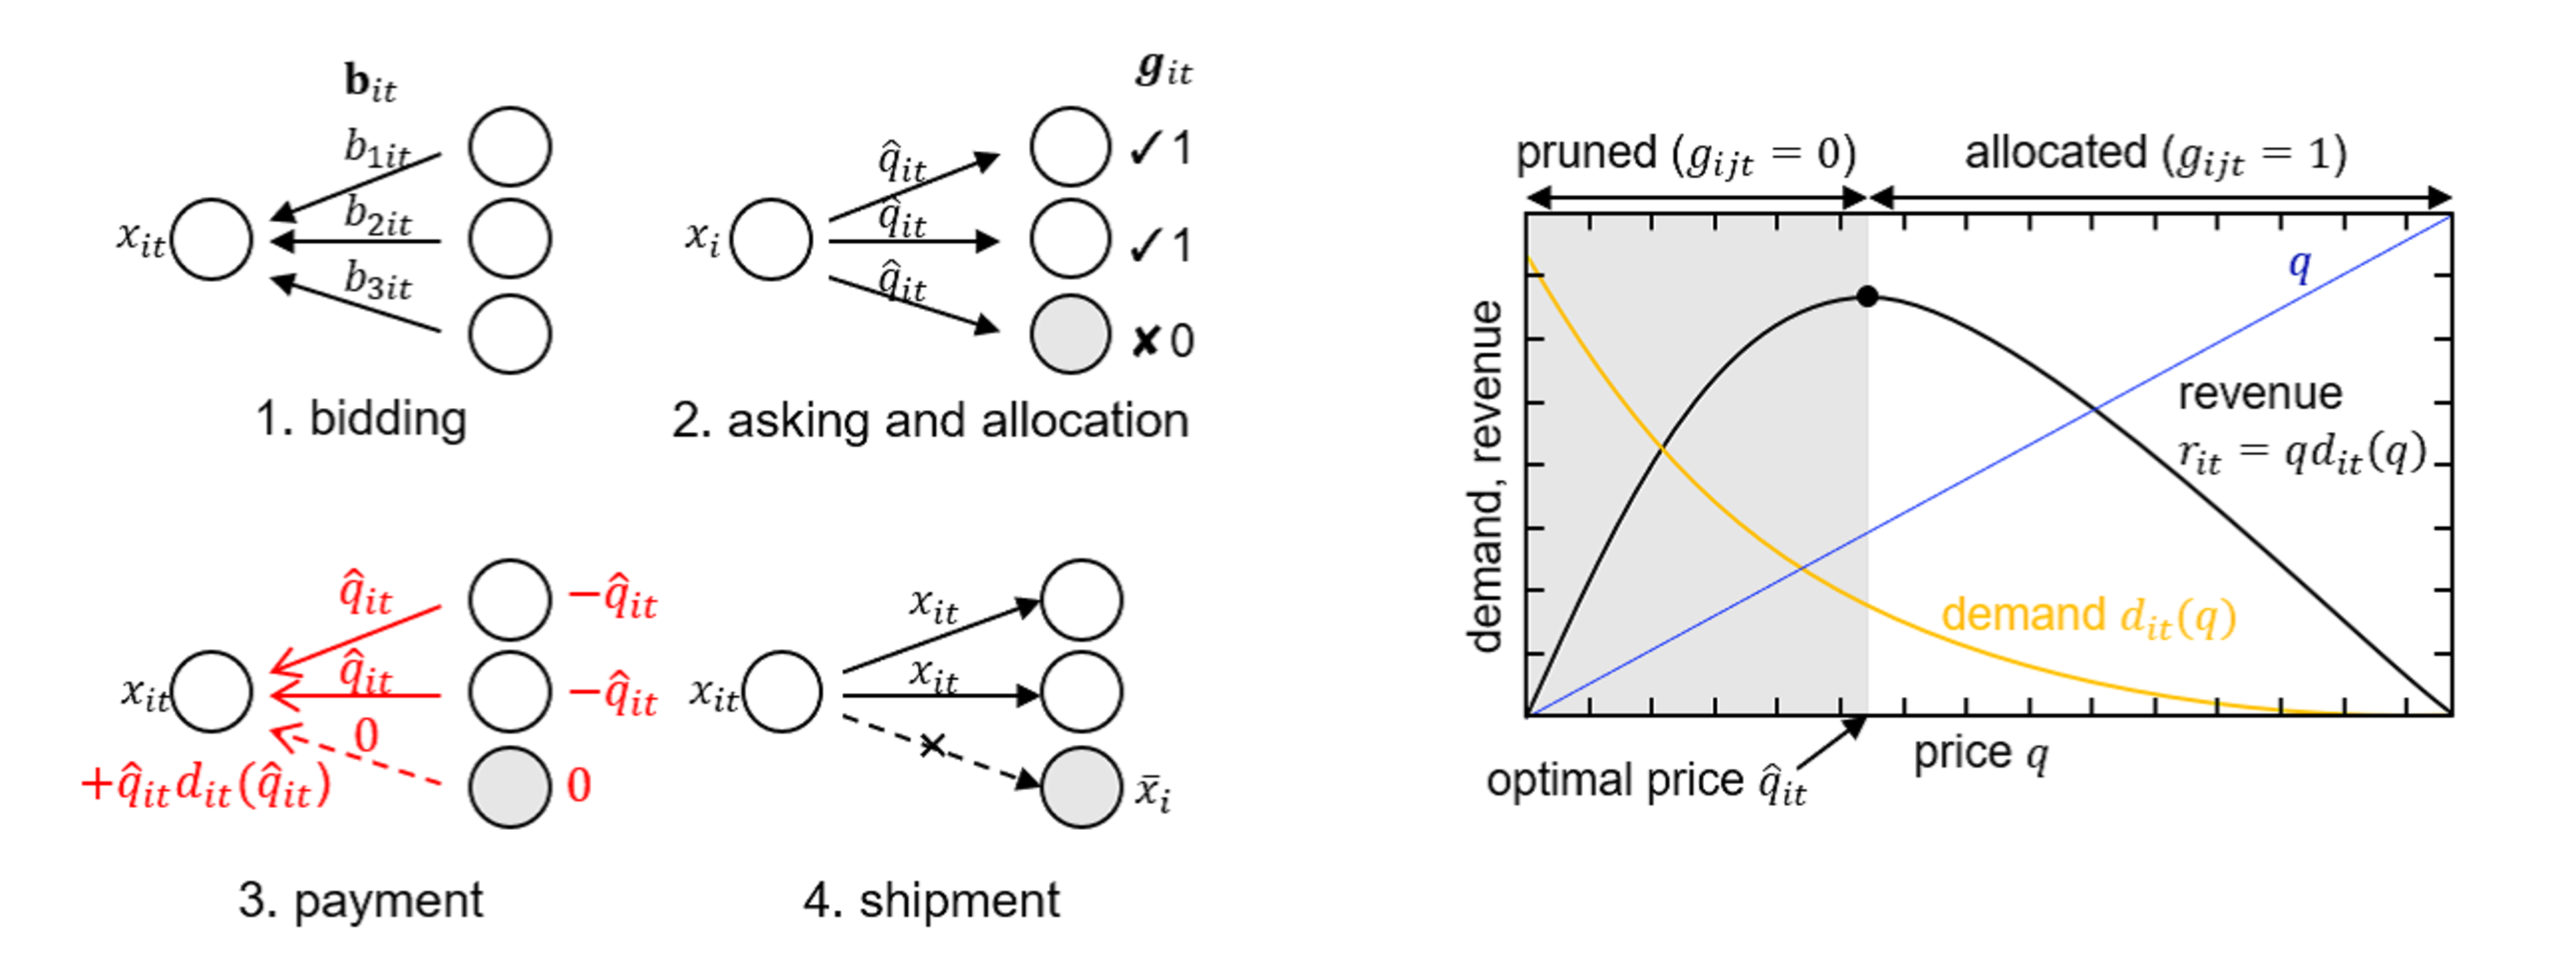
\includegraphics[width=\linewidth]{img/double.eps}
\caption{
\textbf{Left}: The process of trade in an envy-free auction.
\textbf{Right}: A price determination curve for a unit. Revenue of a unit is a product of monotonically decreasing demand and price. The price maximizing the revenue is the optimal price.
}
\label{fig:double}
\end{figure*}


Therefore, the optimization problem is presented below.
\begin{flalign}
	%\max_{\vect{b}, q} \Expect{\hat{\vect{q}}_t}{ V_i^{\pi_i}(s_{it}) } = 
		\max_{\vect{a} } Q_i(s_{it}, \vect{a} )  = 
		\max_q q d_{it}(q) - 
		\min_{\vect{b}} \Expect{\hat{\vect{q}}_t}{\vect{g}_{it}(\vect{b})^\T( \hat{\vect{q}}_t - \gamma \vect{o}_{it}  )} + \const,
		\label{Eq:optimization-probem}
\end{flalign}
where $\vect{a} = (\vect{b}, q)$.
Note that $\vect{g}_{it} = H(\vect{b} - \vect{q}_t)$.
We take the expectation $\Expect{\hat{\vect{q}}_t}{\cdot}$ 
because the asked price $\hat{\vect{q}}_t$ is unknown for $v_i$, except for $\hat{q}_{it}$, and $g_{iit} = 0$.

Then, what is bidding price $b_{it}$ to maximize return?
The following theorem holds.

\begin{thm}\label{thm:optimal-bidding}
	(Truthfulness) the optimal bidding price for maximizing return is $\opt{\vect{b}}_{it} = \gamma \vect{o}_{it}$.
\end{thm}
See the Appendix for the proof.

That is, the unit should only consider its counterfactual return (!).
If $\gamma = 0$, the case is equivalent to a case without auction. Hence, the bidding value raises if each unit consider long-time reward. 
Consequently, in the mechanism of NaaA, the unit obeys as if performing valuation to the other units, 
and declares the value truthfully.

Then, the following corollary holds:
\begin{coro}\label{coro:optimal-bidding}
	The Nash equilibrium of an envy-free auction $(\vect{b}_{it}, q_{it})$ is $(\vect{o}_{it}, \argmax_{q} q d_{it}(q))$.
\end{coro}

The remaining problem is how to predict $\vect{o}_t$.
Although several method can be applied to this problem,
we use $Q$-learning to predict $\vect{o}_t$.
As $\vect{o}_{it}$ is difference of two $Q$s, we approximate each of $Q$.
Other RL such as SARSA and A3C can be employed.
We parametrize the state with a vector $\vect{s}_t$ 
which contains input and weight.
$\epsilon$-greedy policy with $Q$-learning typically suppose that discrete actions
So, as an action, we employ allocation $g_{ijt}$ instead of $\vect{b}_{it}$ and $q_{it}$.
The overall algorithm is shown in Algorithm 1.

\begin{algorithm}[t]
\caption{NaaA: inter-agent reward distribution with envy-free auction}
\begin{algorithmic}[1]
	\FOR{ $t=1$ \TO $T$ }
		\STATE Compute a bidding price for every edge: \textbf{for} $(v_j, v_i) \in \edges$ \textbf{do}\
		$b_{ijt} \leftarrow Q^{\pi_i}( \vect{s}_{it}, \vect{e}_j) - Q^{\pi_i}( \vect{s}_{it}, \vect{0})$ 
		\STATE Compute an asking price for every node: \textbf{for} $\unit \in \units$ \textbf{do}\
		$\opt{q}_{it} \leftarrow \argmax_{q \in [0, \infty)} q d_{it}(q).$
		\FOR{$(v_i, v_j) \in \edges$}
				\STATE Compute allocation: $g_{jit} \leftarrow H(b_{jit} - \opt{q}_{it})$ 
				\STATE Compute the price the agent should pay: $\rho_{jit} \leftarrow g_{jit} \opt{q}_{it}$ 
		\ENDFOR
		\STATE Make a payment: \textbf{for} $\unit \in \units$ \textbf{do}\
		$R_{it} \leftarrow \sum_{j \in N^\mathrm{out}_i} \rho_{jit} 
				- \sum_{j \in N^\mathrm{in}_i} \rho_{ijt},$
		\STATE Make a shipment: \textbf{for} $\unit \in \units$ \textbf{do}\
		$\tilde{x}_{ijt} = g_{ijt} x_{ijt} + ( 1 - g_{ijt} ) \bar{x}_{ijt} $

		\FOR{$\unit \in \units$} 
			\STATE Observe external state $\vect{s}_{it}^{\mathrm ex}$
			\STATE $\vect{s}_{it} \leftarrow (\vect{s}_{it}^{\mathrm ex}, \vect{\tilde{x}}_{it}, \bs{\theta}_i)$,\
				where $\vect{\tilde{x}}_{it} = (\tilde{x}_{i1t}, \dots, \tilde{x}_{int})^\mathrm{T}$ and\
				$\bs{\theta}_i$ is $\unit$'s parameter.
			\STATE Sample action $a_{it}^{\mathrm ex} \sim \pi_i^{\mathrm ex}(\vect{s}_{it})$
			\STATE Receive external reward $R_{it} \leftarrow R_{it} + R_{it}^{\mathrm ex}(a_{it}^{\mathrm ex})$
			\STATE Update $Q^{\pi_i}$ under the manner of $Q$-learning by calculating the time difference (TD)-error 
		\ENDFOR
	\ENDFOR
\end{algorithmic}
\end{algorithm}


%========================================================================
% 【論旨】
% - Q-learning と \epsilon-greedy 方策による強化学習で最適化をする
%	 - 状態を入力と重みを用いてパラメトライズする
%	 - 行動として allocation \g を用いる
%	 - 報酬は profit: revenue と cost の差
%    - つまり、NaaA では結果的に全体としてパフォーマンスが向上するようコネクションを最適化する
% 	 - これはランダムにエッジを落とす dropconnect の拡張であり、より精度向上ができると考えられる。
% - NaaA に基づくネットワーク最適化を adaptive dropconnect と名付ける
%	 - 類似の事例として、過去に提案されている adaptive dropout はこれをより一般化した話
%	 - $\epsilon=0$ の場合には dropconnect と完全に等しくなる
% - Adaptive dropconnect は、強化学習以外にも応用可能
% 	 - 強化学習以外の場合は、報酬として正解に基づく 0/1 の情報を用いて、$gamma = 0$ とする。
% 	 - 実装上は層を入れ替えるだけなので簡単
% - アルゴリズム
%========================================================================

%$\vect{o}_t$ のみ用いた greedy な方策を用いると、
%方策として、$\epsilon$-greedy を用いた
%We use $\epslion-greedy$
%We show that pre $Q$ lead us t
%我々は $\epslion-greedy$ における探索は dropconnect であるため、
%adaptive dropconnect に等しいことを示す。
%
%$\epsilon$
%
%次に、adaptive dropconnect について述べる。
%
%Value of the value function $V(s_{i,t+1})$ depends on $s_{i,t+1}$.
%As we already defined, the internal environment of $v_i$ is a set of connected units,
%and the output of units affect to evaluation from the units, namely, weight of edges.
%As the learning rule of a typical artificial neural network obeys to law of Hebb, 
%the reward becomes lower because weight of unit which do not contribute
%the accuracy of output becomes lower.


\section{Related Work}
NaaA belongs to a class of partially observable stochastic game (POSG) \citep{hansen2004dynamic} because it processes multiple units as agents.
POSG, a class of reinforcement learning with multiple agents in a POMDP environment, presents several research issues, one of which is communication.
Commnet \citep{sukhbaatar2016learning}, which exploits the characteristics of a unit that is agnostic to the topology of other units, employs backpropagation to train multi-agent communication.
Another one is credit assignment.
Instead of reward $R(a_t)$ of an agent $i$ for actions at $t$ $a_t$, 
QUICR-learning \citep{agogino2006quicr} maximizes counterfactual reward $R(a_t) - R(a_t - a_{it})$, the difference in the case of the agent $i$ takes an action $a_{it}$ ($a_t$) and not ($a_t-a_{it}$).
COMA \citep{foerster2017counterfactual} also maximizes counterfactual rewards in an actor--critic setting.
In the setting, all actors have common critics, which improves both actors and critics with time difference (TD)-error of a counterfactual reward.
This paper unifies both issues: communication and credit assignment.
The main proposal is a framework to manage the agents to maximize the {\em counterfactual return}, the extended counterfactual reward along the time axis.

Training a neural network with a multi-agent game is an emerging methodology.
Generative adversarial nets (GAN) \citep{goodfellow2014generative} have the goal of obtaining true generative distribution as a Nash equilibrium of a competitive game that includes two agents with contradictory rewards: a generator and a discriminator. 
In game theory, the outcome maximizing overall reward is named Pareto optimality.
Nash equilibrium is not guaranteed to converge to Pareto optimality. The difference between them is designated as a dilemma.
Because the existence of a dilemma depends on the reward design, methods to resolve dilemmas with good reward design are being investigated: mechanism design \citep{myerson1983mechanism} is also known as inverse game theory.
Mechanism design is applied to auctions \citep{vickrey1961counterspeculation} and matching \citep{gale1962college}.
GAN and our proposal, NaaA, are outcomes from mechanism design.
NaaA applies a digital goods auction \citep{guruswami2005profit} to reinforcement learning with a multi-agent neural network, 
to obtain a maximized return by units as a Nash equilibrium.

%TODO: Dropconnect

\iffalse
・交通ネットワーク - 大澤
・Atari - 田村
・VisDoom - 阿久澤

可能であれば
・ニューロエボリューション

乗せる図
・精度(Learning Curve)
・価値の評価をレイヤーごとに表示
\fi

%\section{Application for Single Agent}
\section{Further Application}
Actually, NaaA is useful not only for multi-agent RL, but also for training of the network.
Typical training algorithms of a neural network such as those of RMSProp \citep{tieleman2012lecture} and Adam \citep{kingma2014adam} are based on a sequential algorithm such as stochastic gradient descent (SGD).
Therefore, the problem can be interpreted as a problem to update the state (i.e., weight) to the goal, which is minimization of the expected likelihood.

The learning can be accelerated by application of NaaA to the optimizer.
We designate the application of NaaA to SGD as {\em Adaptive DropConnect} (ADC), 
which is eventually a combination of DropConnect \citep{wan2013regularization} and Adaptive DropOut \citep{ba2013adaptive}.
We introduce ADC herein as one application of NaaA.

ADC uses NaaA for supervised optimization problem with several revisions.
First, an environment has an input state such as an image. The agent is expected to update its parameters to maximize its reward obtained from the criterion calculator.
The criterion calculator gives batch-likelihood as the reward to the agent.
The agent is a classifier which updates its weights to maximize the reward from the criterion calculator.
The weights are recorded as an internal state.
As a counterfactual return $o_{ijt}$, we used a heuristic that uses the absolute value of weight $|w_{ijt}|$, which is the
same technique as that used by Adaptive DropOut.
We use the absolute value of weights because it is the update amount for which the magnitude of error of the output of units is proportional to $|w_{ijt}|$.

The algorithm is presented as Algorithm 2.
Because the algorithm is quite simple, its implementation can be performed easily.
For that reason, it can be widely applied for most general deep learning problems such as 
image recognition, sound recognition, and even for deep reinforcement learning.

\begin{algorithm}[t]
\caption{Adaptive DropConnect}
\begin{algorithmic}[1]
	\FOR{ $t=1$ \TO $T$ }
		\STATE Compute a bidding price for every edge: \textbf{for} $(v_j, v_i) \in \edges$ \textbf{do} \
		$b_{ijt} \leftarrow |w_{ijt}|$ 
		\STATE Compute an asking price for every node: \textbf{for} $\unit \in \units$ \textbf{do} \
		$\opt{q}_{it} \leftarrow \argmax_{q \in [0, \infty)} q d_{it}(q).$
		\FOR{$(v_i, v_j) \in \edges$}
				%\STATE Sample $u$ from a Bernoulli distribution: $u \sim \mathrm{Bernoulli}(\varepsilon)$
				%\STATE Sample $m$ from a Bernoulli distribution: $m \sim \mathrm{Bernoulli}(1/2)$
				\STATE Compute allocation: $g_{jit} \leftarrow H(b_{jit} - \opt{q}_{it})$ 
		\ENDFOR
		\STATE Sample a switching matrix $U_t$ from a Bernoulli distribution: $U_t \sim \mathrm{Bernoulli}(\varepsilon)$
		\STATE Sample the random mask $M_t$ from a Bernoulli distribution: $M_t \sim \mathrm{Bernoulli}(1/2)$
		\STATE Generate the adaptive mask: $M_t' \leftarrow U_t \circ M_t + (1 - U_t) \circ G_{ijt}$ 
		\STATE Compute $\vect{h}_t$ for making a shipment:
			$\vect{h}_t \leftarrow (M_t' \circ W_t) \vect{x}_t + \vect{b}_t$
		\STATE Update $W_t$ and $\vect{b}_t$ by backpropagation.
	\ENDFOR
\end{algorithmic}
\end{algorithm}

\subsection{Experiment}

\subsubsection{Setup}
In this experiment, we confirm two tasks of classification and single-agent reinforcement learning.

For classification task, we used three types of datasets, MNIST, CIFAR-10 and STL-10. 
The task given here is to predict the label for each image. The number of class is 10 in those three datasets.
The first dataset, MNIST, is a collection of black and white images of handwritten digits whose size is 28x28. The training set and test set are composed of 60,000 examples and 10,000 examples respectively. 
The images in CIFAR-10 dataset are colored and the size of each image is 32x32. The task is to predict what is shown in each picture. This dataset contains 6,000 images per class (5,000 for training and 1,000 for test).
STL-10 is a dataset for image recognition, the number of which is 1,300 for each class (500 for training and 800 for test). The size of each image is 96x96. In this experiment, however, images were resized into 48x48, since the resolution is large compared to the datasets shown above and this dataset requires far more time and resource to compute.

Next, we set the single-agent reinforcement learning task.
We used the CartPole task from OpenAI gym with visual input.
In this setting, the agent must balance a pole while moving a cart.
There is much non-useful information related to the image. For that reason, pruning the pixels is important.

\subsubsection{Model}
In this experiment, we compared two models, DropConnect and Adaptive DropConnect (proposed model in this paper). The baseline model is composed of two convolutional layers and two fully connected layers whose outputs are dropped out (we set the possibility as 0.5). The labels of input data are predicted using log-softmaxed value of last fully connected layer. In DropConnect model and Adaptive DropConnect model, first fully connected layer is replaced by DropConnected layer  and Adaptive DropConnected layer respectively. Note that DropConnect model corresponds to the our method with $\varepsilon$ = 1.0 and this means agents do not perform their auctions, and randomly mask the weights.

\subsubsection{Results}
For the MNIST datasets, the models are trained for 10 epochs and then evaluated with the test data. The numbers of epochs for CIFAR-10 and STL-10 are 20 and 40 respectively. Experiments are repeated 20 times for each condition, and the average and standard deviation of  error rate was calculated. The results is shown in Table \ref{tbl:cls}. As expected, with the model using Adaptive DropConnect, the classification error rate was lower than both the baseline and DropConnect regardless of the datasets given in this experiment.


\begin{table}[h]
	\caption{ Experimental result for image classification tasks and single-agent RL }\label{tbl:cls}. 
\centering
\begin{tabular}{l|ccc|c}
\hline
		& MNIST & CIFAR-10 & STL-10 & CartPole \\
\hline
		DropConnect \citep{wan2013regularization}	&	1.72 $\pm$ 0.160	&	43.14 $\pm$ 1.335	&	50.92 $\pm$ 1.322 & 285 \\
		Adaptive DropConnect	&	\textbf{1.36} $\pm$ 0.132	&	\textbf{39.84} $\pm$ 1.035	&	\textbf{42.17} $\pm$ 2.329 & \textbf{347} \\
\hline
\end{tabular}
\end{table}


\section{Discussion}
\subsection{Disadvantage}
The one of disadvantage is computational complexity.
As envy-free auction uses sort operation for computing demand,
several part should be serialized.
It should be improved with Approximation.

For optimization method,
although envy-free auction guarantees truthfulness if the prices of buyer are sealed,
in the case which buyer can communicate each other and shares price information, 
the buyer can fake the price with lower demand in collusion.
For the issue, several solution such as random sample auction \cite{goldberg2006competitive} is proposesd.

Adoptive dropconnect has difficulty for implementation for several neural network.
Although, we published source code on GitHub for Linear and CNN, 
implementation for RNN is a future work.

\subsection{Application}
NaaA can be applied on learning distributed environment on computer network such as peer-to-peer network, and controlling sub-module of robot such as multiple camera.
Specifically, it can be applied to various method as below.
\begin{itemize}
\item Hyperparameter tuning. 
Several algorihtm are already proposed such as neuroevolution using genetic algorithm.
In the case, profit or counterfactual return can be used to fitness function.

\item Pruning. Reducing computing cost with downsizing neural network.
\item Attention control. In a part of research of attention, they are using reinforcement learning to control attention.
\item Ensamble. Our method can be applied to mix multiple models.
\end{itemize}
These application is direction of the research.

%\section{Conclusion and Future Works}
\section{Concluding Remarks and Future Work}
This paper proposed a NaaA model to address communication in MARL without a TTP based on two key ideas: inter-agent reward distribution and auction theory.
Existing MARL communication methods have assumed the existence of a TTP, and hence could not be applied in peer--to--peer environments.
The inter-agent reward distribution, making agents redistribute the rewards they received from the internal/external environment, was reviewed first.
When an envy-free auction was introduced using auction theory, it was shown that agents would evaluate the counterfactual returns of other agents.
The experimental results demonstrated that NaaA outperformed a baseline method and a CommNet-based method.

Furthermore, a $Q$-learning based algorithm, termed Adaptive DropConnect, was proposed to dynamically optimize neural network topology with counterfactual return evaluation as a further application.
To evaluate this application, experiments were performed based on a single-agent platform, demonstrating that the proposed method produced improved experimental results relative to existing methods.

% TODO: ���������ꍇ�̑΍�͂ǂ����ɏ���������������������Ȃ�

Future research may also be directed toward considering the connection between NaaA and neuroscience or neuroevolution.
Edeleman propounded the concept of neural Darwinism \citep{edelman1987neural}, in which group selection occurs in the brain.
Inter-agent rewards, which were assumed in this paper, correspond to NTFs
and could be used as a fitness function in genetic algorithms for neuroevolution such as hyperparameter tuning.

As NaaA can be applied in peer-to-peer environments, 
the implementation of NaaA in blockchain \citep{swan2015blockchain} is under consideration.
This implementation would extend the areas where deep reinforcement learning could be applied.
Bitcoin \citep{nakamoto2008bitcoin} could be used for inter-agent reward distribution, and the auction mechanism could be implemented by smart contracts \citep{buterin2014next}.
Using the NaaA reward design, it is hoped that the world may be united, allowing people to share their own representations on a global scale.

%We can use bitcoin \cite{nakamoto2008bitcoin} and smart contract \cite{}a 

%Besides, we proposed Adaptive DropConnect as an further application on a single neural network.
%This paper proposed NaaA, a reinforcement learning framework that treats each unit on a neural network as an agent.
%First, we pointed out there are dilemma problems if we naively optimize NaaA. 
%We proposed an optimization method with auction.
%Consequently, an action by which units evaluate the counterfactual return of other units is obtained as a Nash equilibrium.
%Furthermore, we proposed $Q$-learning based algorithm, adaptive dropconnect, to optimize the neural network topology dynamically with evaluation of counterfactual return.
%For the evaluation, we performed experiments based on single-agent and multi-agent platforms, demonstrating that our experimentally obtained results improve existing methods.

%As a direction of future research, we use on-policy methods to perform adaptive dropconnect, and
%consider applications combining genetic algorithms.


\bibliography{daisy}
\bibliographystyle{iclr2018_conference}

\appendix
\section*{Appendix}

% Set numbering of section alphabet: A, B, C,...
\setcounter{section}{1}
\renewcommand{\thesection}{\Alph{section}}

% Contents is started from here
%\subsection{Proof}
%We first proof $\rho_{ijt} = 0$ is the Nash equilibrium.
%The value function can be written as $r_{it} - c_{it} + \gamma V_{i,t+1}$.
%At the point, as other agents plays $\rho_{ijt} = 0$, the value function is $- c_{it}$.
%To maximizing this equation, $\rho_{ijt} = 0$ holds. 

\subsection{Proof of Theorem \ref{thm:optimal-bidding}}
%As for a buyer, the asking price $\ask$ for a seller is unknown,
%we address $\ask$ which has support $[0, \infty)$,
%and consideration to maximize $\Expect{q}{G(b,q)}$,
%In this case, the following equation holds.
%\begin{flalign}
%\deriv{b}{}\Expect{q}{G(b,q)} 
%&= \deriv{b}{}\int_0^\infty (H(b - q) \cdot (v-q) + G_0) p(q) dq \notag \\
%&= \deriv{b}{} \left[ \int_0^b (v-q) p(q) dq + G_0 \int_0^\infty p(q)dq \right] \notag \\
%&= \deriv{b}{} \int_0^b (v-q) p(q) dq \notag \\
%&= (v-b) p(q=b), \notag 
%\end{flalign}
%Therefore, the condition to maximize $\Expect{q}{G(b,q)}$ is $b=v$.

The optimization problem in Eq:\ref{Eq:optimization-probem} is made of two terms except of the constant, 
and the only second term is depends on $\vect{b}$.
Hence, we consider to optimize the second term.
The optimal bidding prices $\hat{\vect{q}}_t$ is given by the following equation.

\begin{flalign}
\hat{\vect{b}}_{it} 
&= \argmin_{\vect{b}} \Expect{\vect{q}_t}{\vect{g}_{it}(\vect{b})^\T( \vect{q}_t - \gamma \vect{o}_{it}  )} 	
= \argmin_{\vect{b}} \Expect{\vect{q}_t}{H(\vect{b} - \vect{q}_{t})^\T ( \vect{q}_t - \gamma \vect{o}_{it}  )}	\notag \\
&= \argmin_{\vect{b}} \Expect{\vect{q}_t}{\sum_{j=1}^N H(b_{j} - q_{jt}) ( q_{jt} - \gamma o_{ijt}  )}		
= \argmin_{\vect{b}} \sum_{j=1}^N \Expect{q_{jt}}{H(b_{j} - q_{jt}) ( q_{jt} - \gamma o_{ijt}  )},
\end{flalign}

From independence, the equation is solved if we solve the following problem.

\begin{flalign}
\hat{b}_{ijt} = \argmin_{b} \Expect{q_{jt}}{H(b - q_{jt}) ( q_{jt} - \gamma o_{ijt}  )}, \, \, \, \forall j \in \{1, \dots, N\}
\end{flalign}

Hence, $\hat{b}_{ijt}$ can be derived as the solution which satisfies the following equation. 
\begin{flalign}
	\left. \deriv{b}{}\Expect{q_{jt}}{H(b - q_{jt}) ( q_{jt} - \gamma o_{ijt}  )} \right|_{b=\hat{b}_{ijt}}  = 0,  \, \, \, 
\left. \derivN{2}{b}{}\Expect{q_{jt}}{H(b - q_{jt}) ( q_{jt} - \gamma o_{ijt}  )}\right|_{b=\hat{b}_{ijt}} > 0 \notag 
\end{flalign}

For simplicity, we let $q = q_{jt}$ and $o = o_{ij,t+1}$. Then, the following equation holds.

\begin{flalign}
\deriv{b}{}\Expect{q}{H(b - q)( q - \gamma o  )} 
&= \deriv{b}{}\int_0^\infty H(b - q)(q - \gamma o) p(q) dq \notag \\
&= \deriv{b}{} \int_0^b (q - \gamma o) p(q) dq \notag \\
	&= (b-\gamma o) p(q=b), \label{eq:deriv1}
\end{flalign}
\begin{flalign}
	\derivN{2}{b}{}\Expect{q}{H(b - q)( q - \gamma o  )} = p(q=b) + (b - \gamma o) \deriv{b}{}p(q=b)  \label{eq:deriv2}
\end{flalign}

Then, condition $\deriv{b}{}\Expect{q_{jt}}{H(b - q_{jt}) ( q_{jt} - \gamma o_{ijt}  )} |_{b=\hat{b}_{ijt}}  = 0$ is satisfied only by $\hat{b}_{ijt} = \gamma o_{ijt}$.
We substitue $\hat{b}_{ijt}$ into Eq:\ref{eq:deriv2},
\begin{flalign}
\left. \derivN{2}{b}{}\Expect{q_{jt}}{H(b - q_{jt}) ( q_{jt} - \gamma o_{ijt}  )}\right|_{b=\hat{b}_{ijt}} 
	&= p(q=\hat{b}_{ijt}) + 0 > 0
\end{flalign}

Therefore, $\hat{b}_{ijt} = \gamma o_{ijt}$ is a unique solution as the minimum point.
From generality, $\hat{\vect{b}}_{it} = \gamma \vect{o}_{it}$ holds.


\end{document}
